%%%%%%%%%%%%%%%%%%%%%%%%%%%%%%%%%%
\section{Results using $k_T$-factorization approach}
%%%%%%%%%%%%%%%%%%%%%%%%%%%%%%%%%%
%------------------------------------------------------------------------------------


Several different parametrizations of proton strucure functions are used. Those are labeled as:
%%
\begin{itemize} 

 \item ALLM \cite{Abramowicz:1991xz,Abramowicz:1997ms}: This parametrization gives a good fit to $F_2$ in most of the measured regions.
   
  
\item SY \cite{Suri:1971yx}: This parameterization of Suri and Yennie from the early 1970's does not include DGLAP evolution. It is still  used as one of the defaults in the LPAIR event generator~\cite{Vermaseren:1982cz}.
    
\item SU \cite{Szczurek:1999rd}: A parametrization which concentrates to give a good description at small and intermediate $Q^2$ for $x > 0.01$.
At large $Q^2$, it is complemented by the NNLO calculation of $F_2$ and $F_L$ from NNLO MSTW 2008 PDF analysis~\cite{Martin:2009iq}.
   
\item LUX-like: a recently constructed parametrization, described in details in Ref.~\cite{Luszczak:2018ntp}.
This setup closely follows the LUXqed work from Ref.\cite{Manohar:2017eqh}.
\end{itemize} 

To model $\gamma^{p}_{el}(x, Q^2)$ we use Eq.~\ref{proton_el_flux} with so-called dipole parametrization of the proton form factors:
\begin{eqnarray}
G_E(Q^2) &=& \left( 1+\frac{Q^2}{Q_0^2} \right)^{-2} \\
G_M(Q^2) &=& \mu_p G_E(Q^2)~,
\end{eqnarray}
where $\mu_p$ is the proton magnetic moment.

Table~\ref{tab:kt} shows the comparison of integrated fiducial cross sections for inelastic $p+\textrm{Pb}\rightarrow \textrm{Pb} + \ell^+\ell^- + X$ production at $\sqrt{s_{N N}} = 8.16$~\TeV\ for different proton structure functions.
All structure functions provide similar fiducial cross-section, at the level of 16--18 nb.
These inelastic cross-sections are also similar in size to the elastic contribution (18 nb) and are slightly lower than the numbers from collinear analysis, subtracted for elastic part (see Table~\ref{fig:xs}).
A comparison is also made with LUX-like parametrization when the longitudinal structure function ($F_L$) is explicitly considered.
This leads to the decrease of the cross section by 2\%, similarly to Ref.~\cite{Luszczak:2018ntp}.

Figure~\ref{fig:kt_figures1} presents differential cross sections for several lepton kinematic distributions: invariant mass of lepton pair, leading lepton transverse momentum, lepton pseudorapidity difference and leading lepton pseudorapidity.
The shapes of the distributions obtained with various proton structure functions are very similar.
For completeness, differential cross sections as a function of lepton pair transverse momentum and azimuthal angle difference between the pair  are shown in Fig.~\ref{fig:kt_figures2}. Quite large (small) transverse momenta (angle differences) are possible, in contrast to leading-order calculations with collinear photons where the corresponding distributions are just Dirac delta functions. 
The $k_T$-factorization approach should be considered more appropriate here. It is also visible that the SY parametrization gives lower predictions at larger pair-$p_T$, comparing to the other parametrizations used. This is because SY parametrization does not include explicit DGLAP evolution terms, which are relevant for large photon virtualities.

Based on Fig.~\ref{fig:kt_figures2}, it is also possible to separate experimentally the elastic part ($p+\textrm{Pb}\rightarrow p+ \textrm{Pb} + \ell^+\ell^-$), with striking back-to-back topology, from the inelastic contribution.
With $k_T$-factorization, one can also calculate the mass of the proton remnants ($M_X$). This is shown in Fig.~\ref{fig:kt_figures3}; in contrast to the elastic case ($M_X=m_p$) quite large masses of the remnant system can be achieved.



\begin{table}[t]
\centering
\begin{tabular}{|l|c|c|c|}
\hline
Contribution  &  $p_{T}^{\ell}>4~\GeV$ & $p_{T}^{\ell}>4~\GeV$, $|\eta^{\ell}|<2.4 $, $m_{\ell^+\ell^-}>10~\GeV$ \\
\hline
$\gamma^{p}_{\rm{el}}$   & 47.9 nb  & 18.3 nb \\
\hline
$\gamma^{p}_{\rm{inel}}$ [LUX-like  $F_2$]  & 43.6 nb  &  17.4 nb\\
\hline
$\gamma^{p}_{\rm{inel}}$ [LUX-like  $F_2+F_L$]  & 42.6 nb    & 17.1 nb\\
\hline    
$\gamma^{p}_{\rm{inel}}$ [ALLM97 $F_2$]  & 41.7 nb   &16.4 nb\\
\hline
$\gamma^{p}_{\rm{inel}}$ [SU $F_2$]  & 41.7  nb &16.7 nb\\
\hline 
$\gamma^{p}_{\rm{inel}}$ [SY $F_2$]  & 40.4  nb  &16.0 nb\\
\hline
\end{tabular}
\caption{Integrated fiducial cross sections for inelastic $p+\textrm{Pb}\rightarrow \textrm{Pb} + \ell^+\ell^- + X$ production at $\sqrt{s_{N N}} = 8.16$~\TeV\ for different proton structure functions. 
The effect of applying only $p_T^{\ell}$ requirement is shown in second column.
}
\label{tab:kt}
\end{table}



%-----------------------------------------------------------------------------
\begin{figure}[!h]
 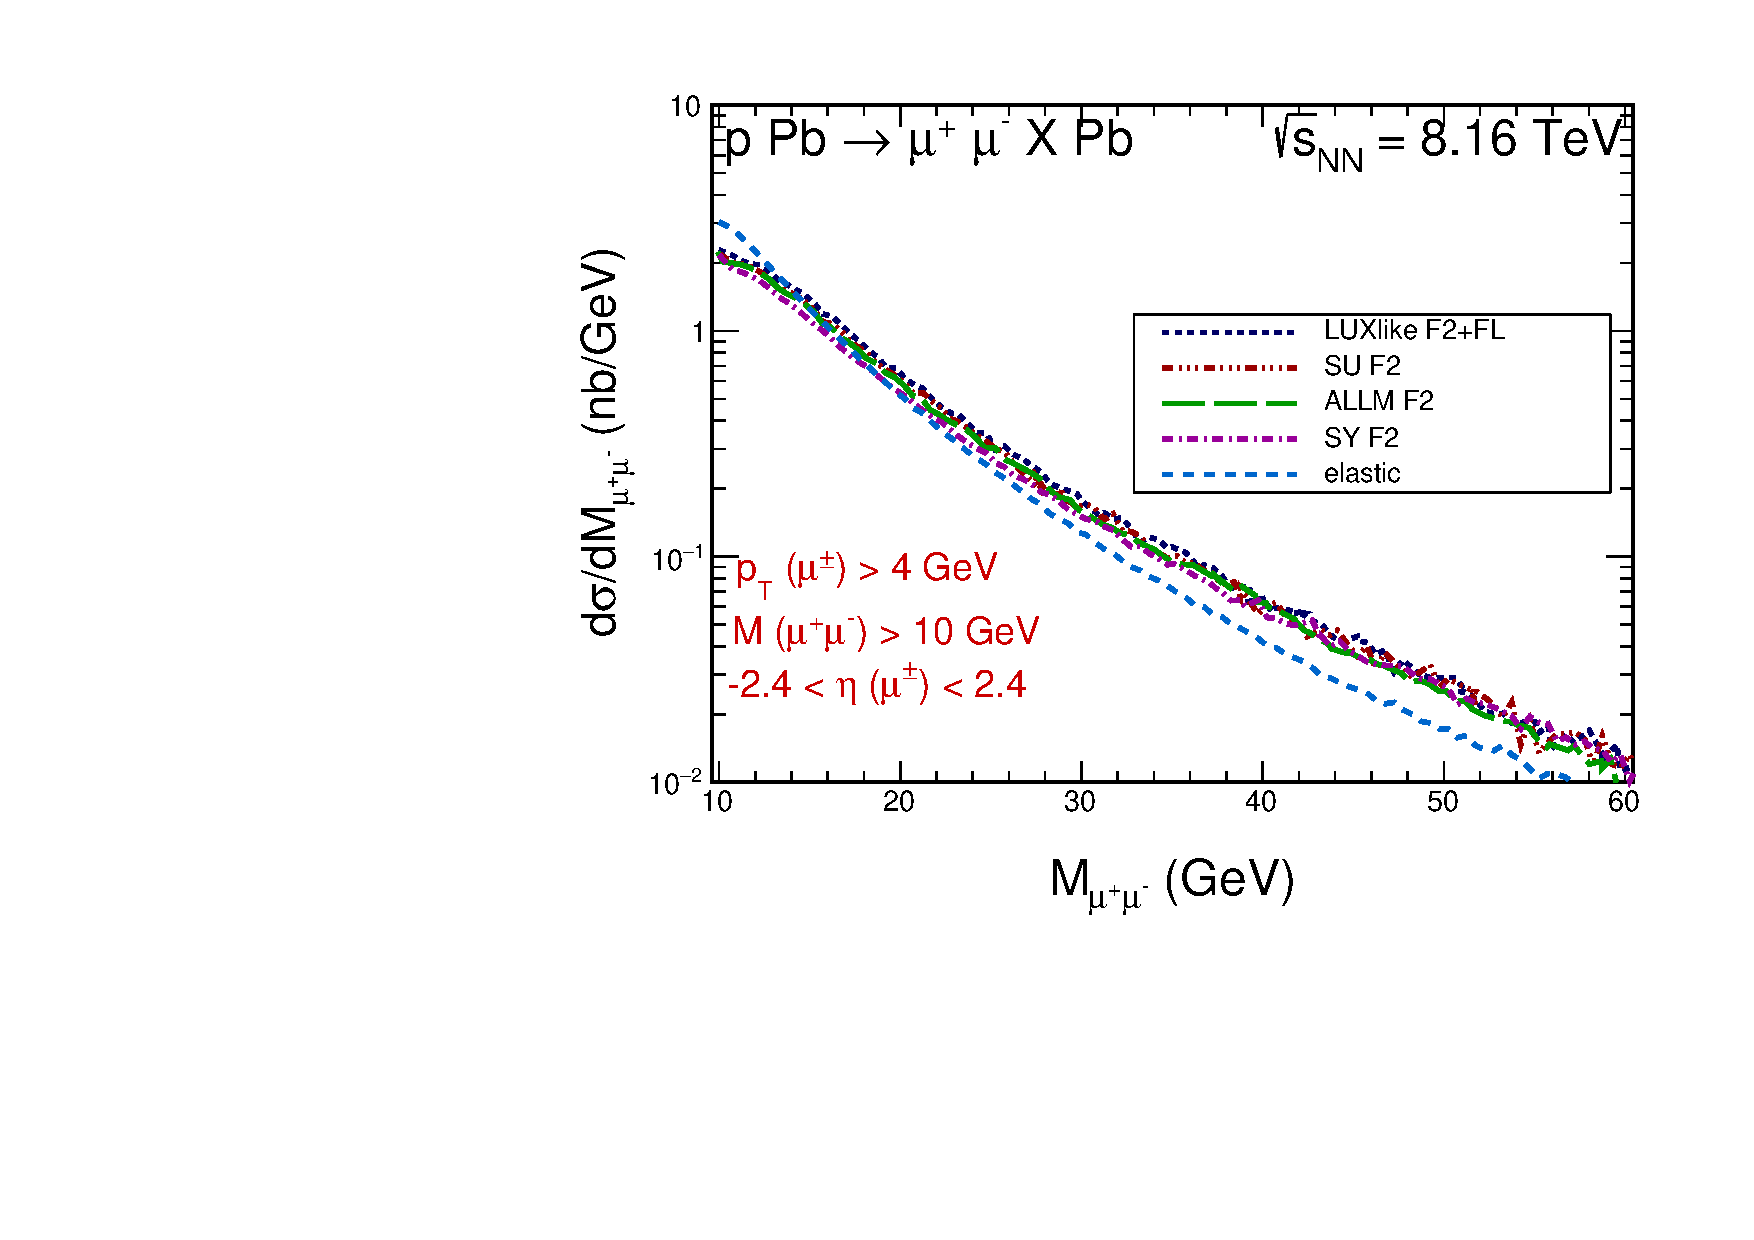
\includegraphics[width=0.49\textwidth]{figures/Mll-l.pdf}
  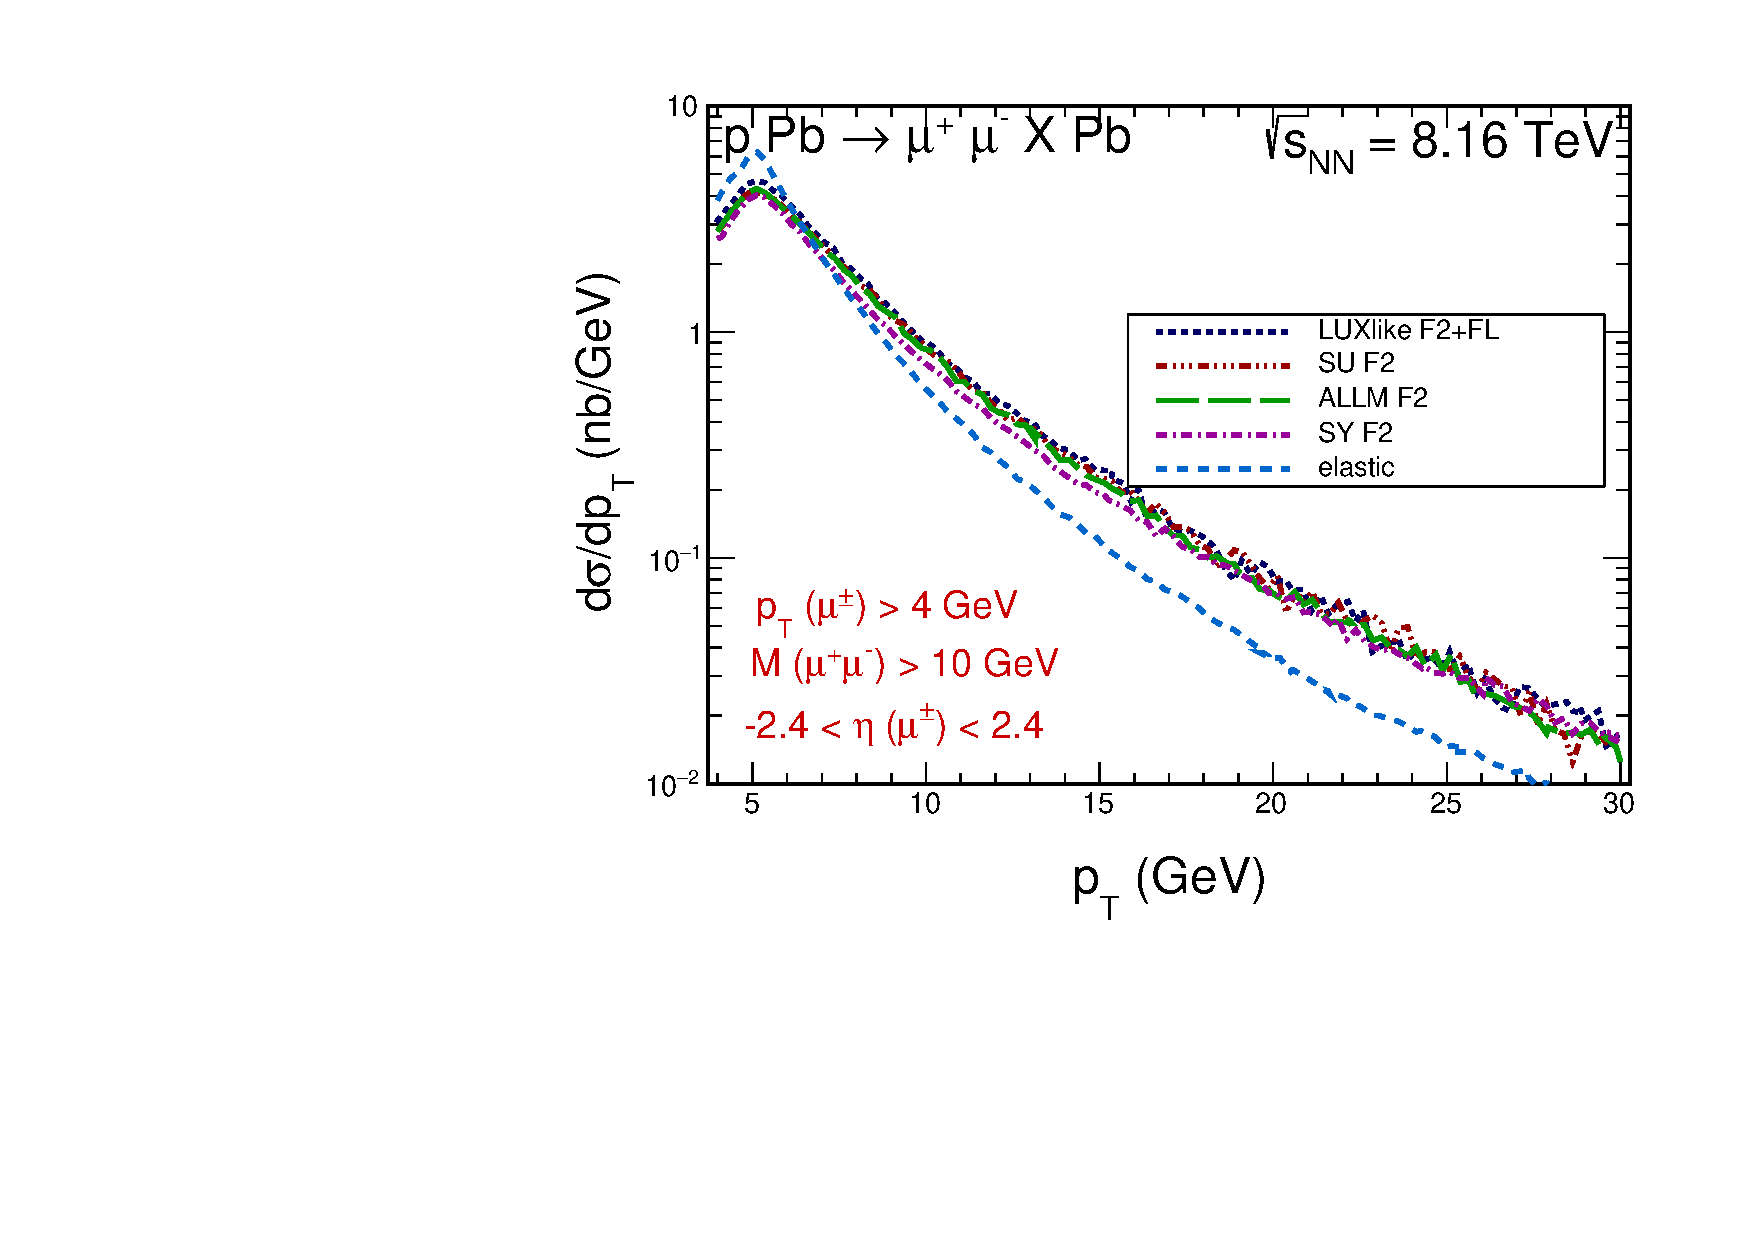
\includegraphics[width=0.49\textwidth]{figures/pt1-l.pdf}
 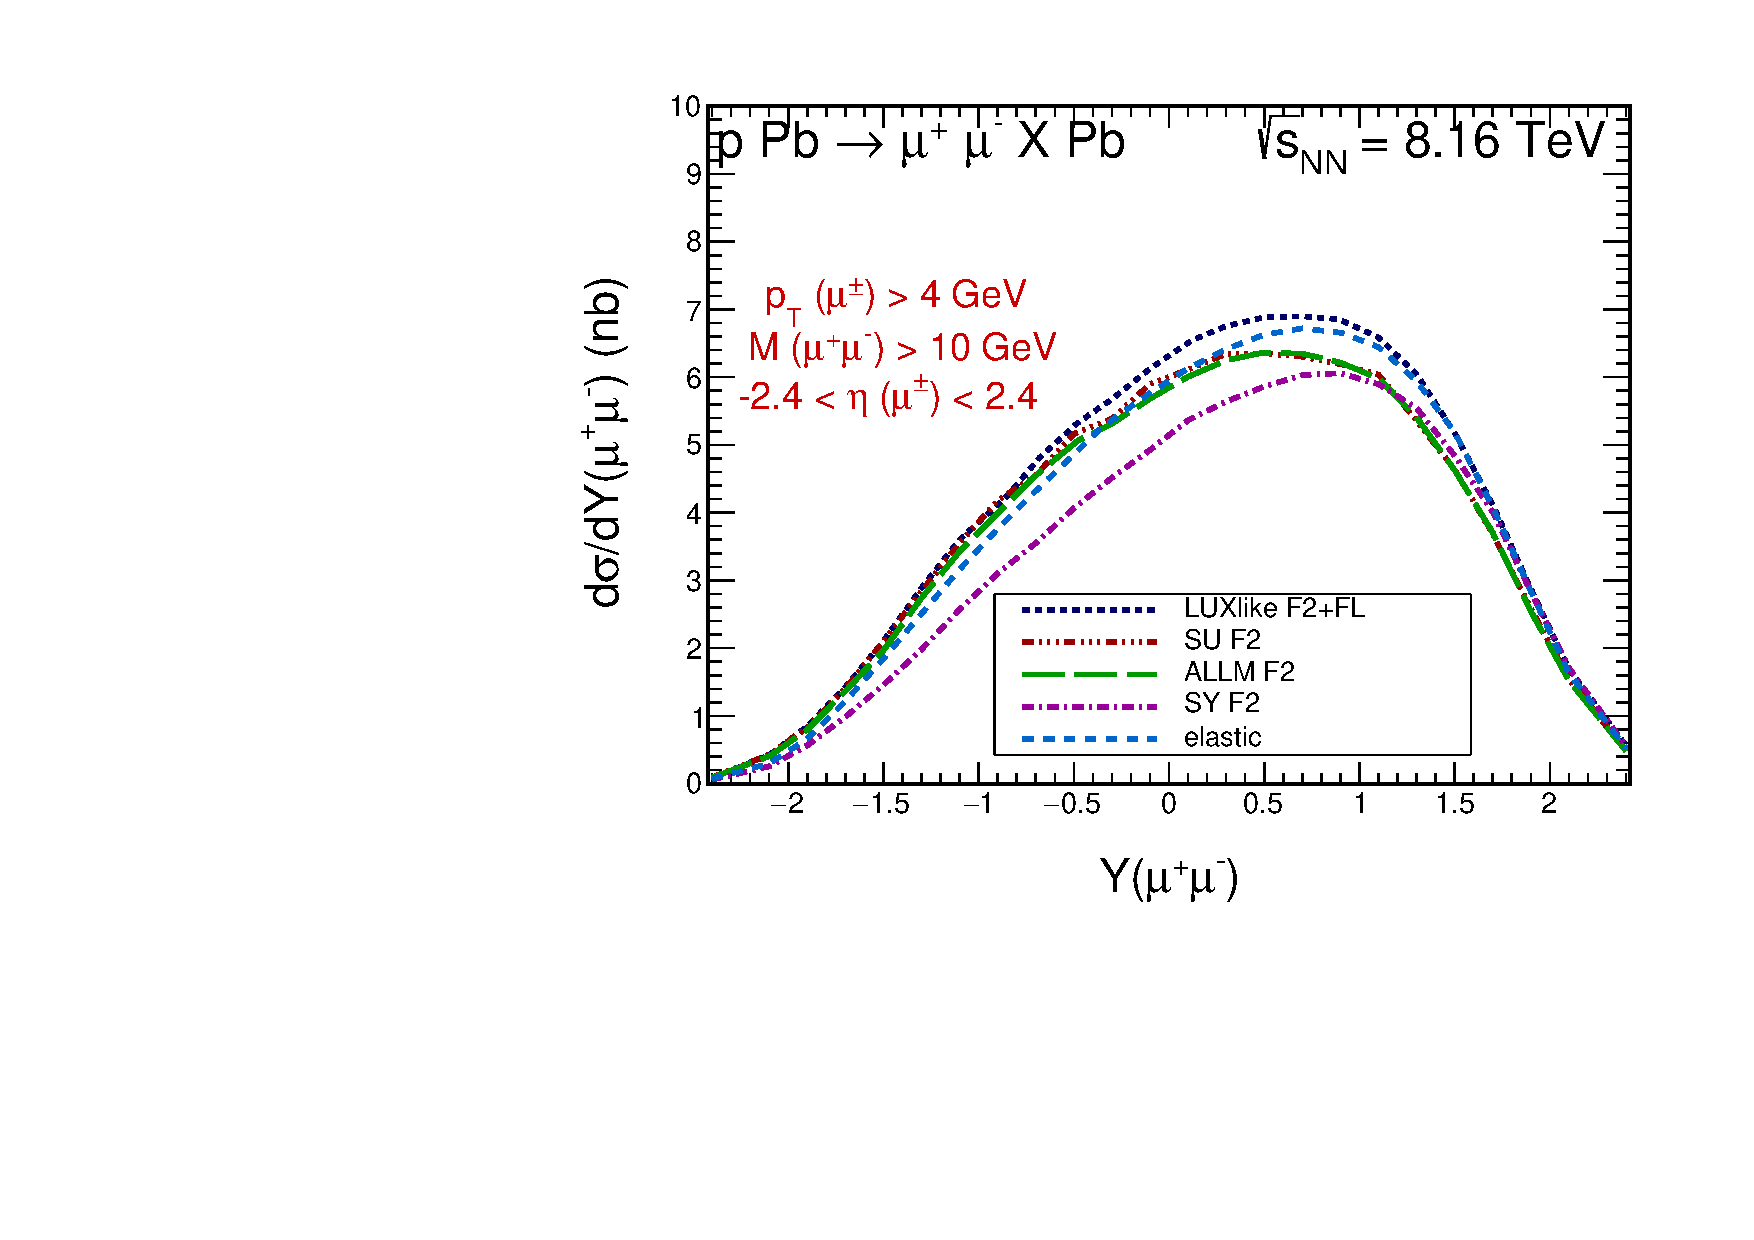
\includegraphics[width=0.49\textwidth]{figures/Y-l.pdf}
  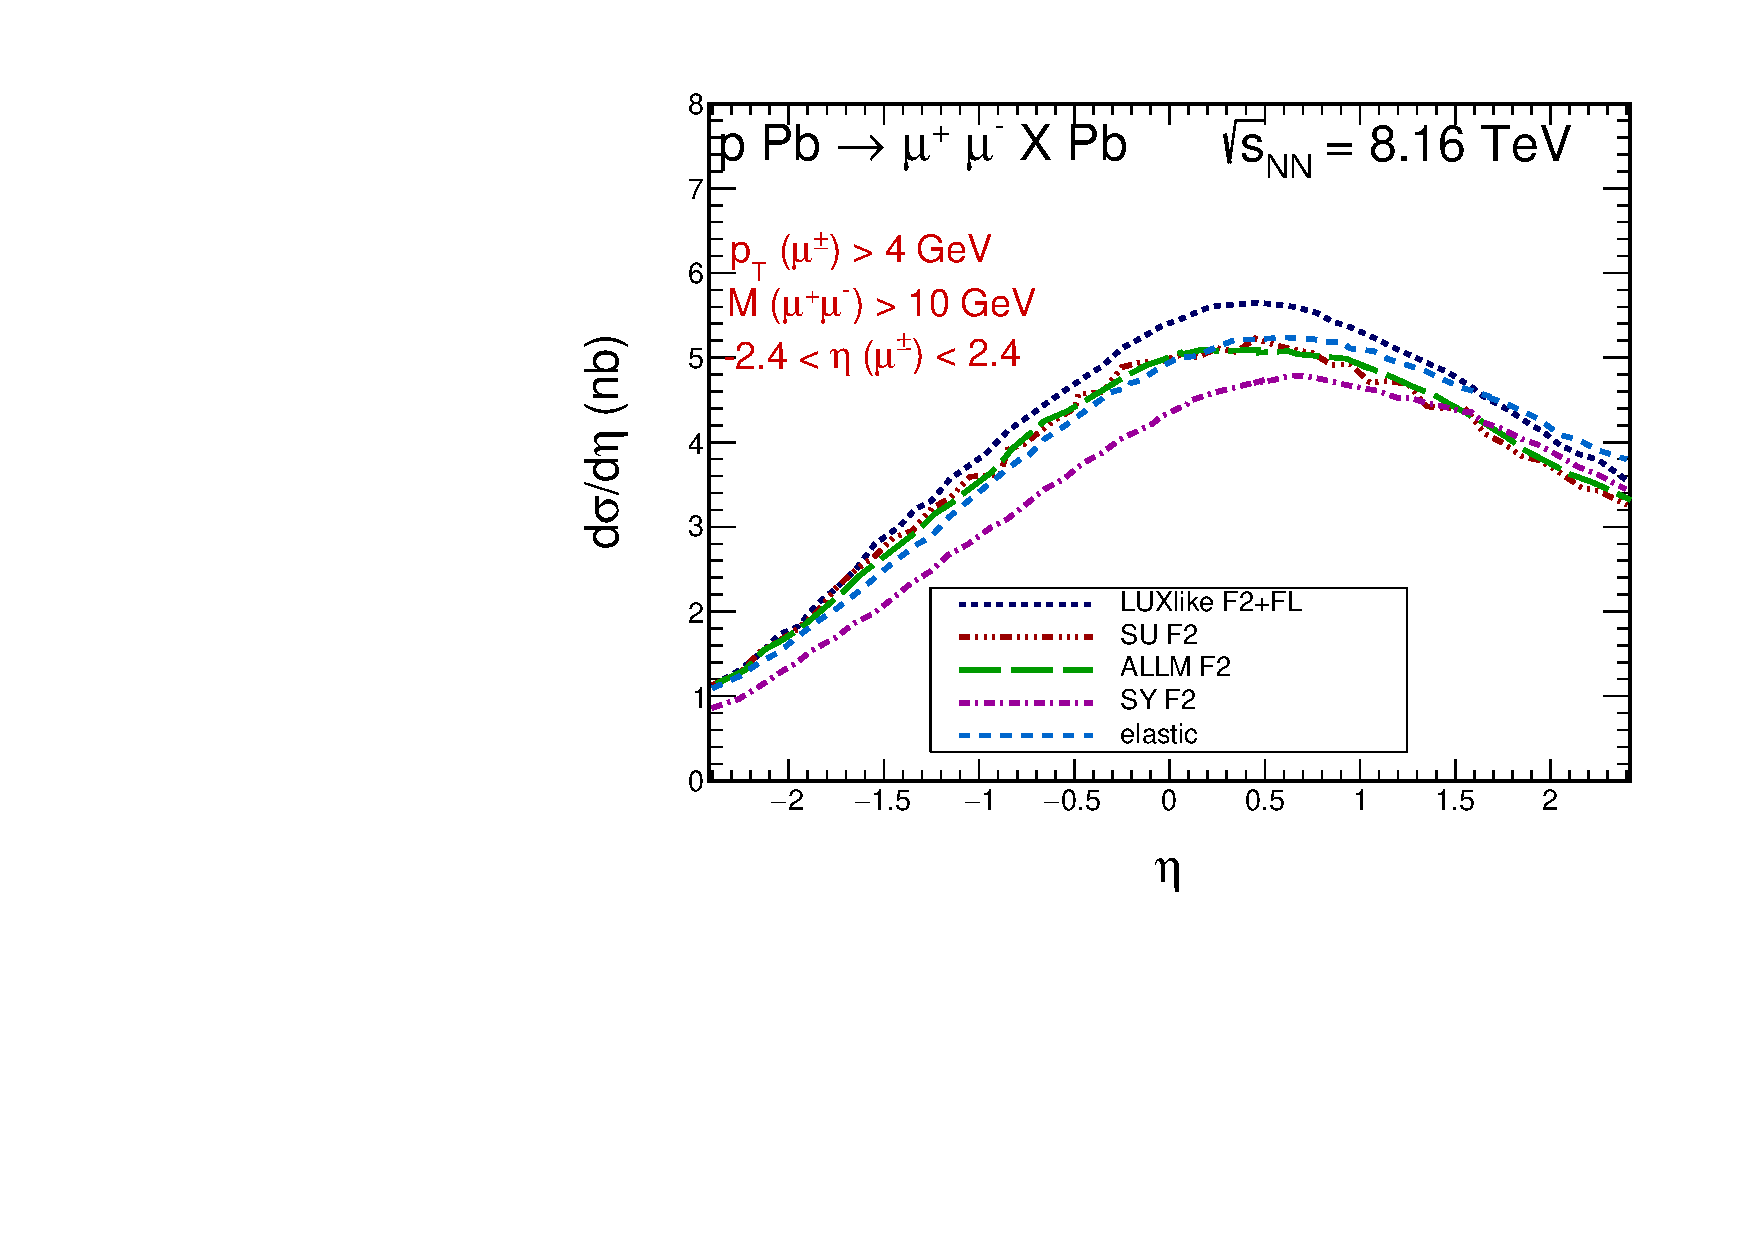
\includegraphics[width=0.49\textwidth]{figures/y1-l.pdf}
\caption{Differential cross sections in the fiducial region for $p+\textrm{Pb}\rightarrow \textrm{Pb} + \ell^+\ell^- + X$ production at $\sqrt{s_{N N}} = 8.16$~\TeV\ in $k_T$ factorization approach for several proton structure functions.
Four differential distributions are shown: invariant mass of lepton pair (top left), leading lepton transverse momentum (top right),
dilepton rapidity (bottom left) and leading lepton pseudorapidity (bottom right).
For comparison, the elastic contribution ($p+\textrm{Pb}\rightarrow p+ \textrm{Pb} + \ell^+\ell^-$) is also shown.
}
 \label{fig:kt_figures1}
\end{figure}
%------------------------------------------------------------------------------


%-----------------------------------------------------------------------------
\begin{figure}[!h]
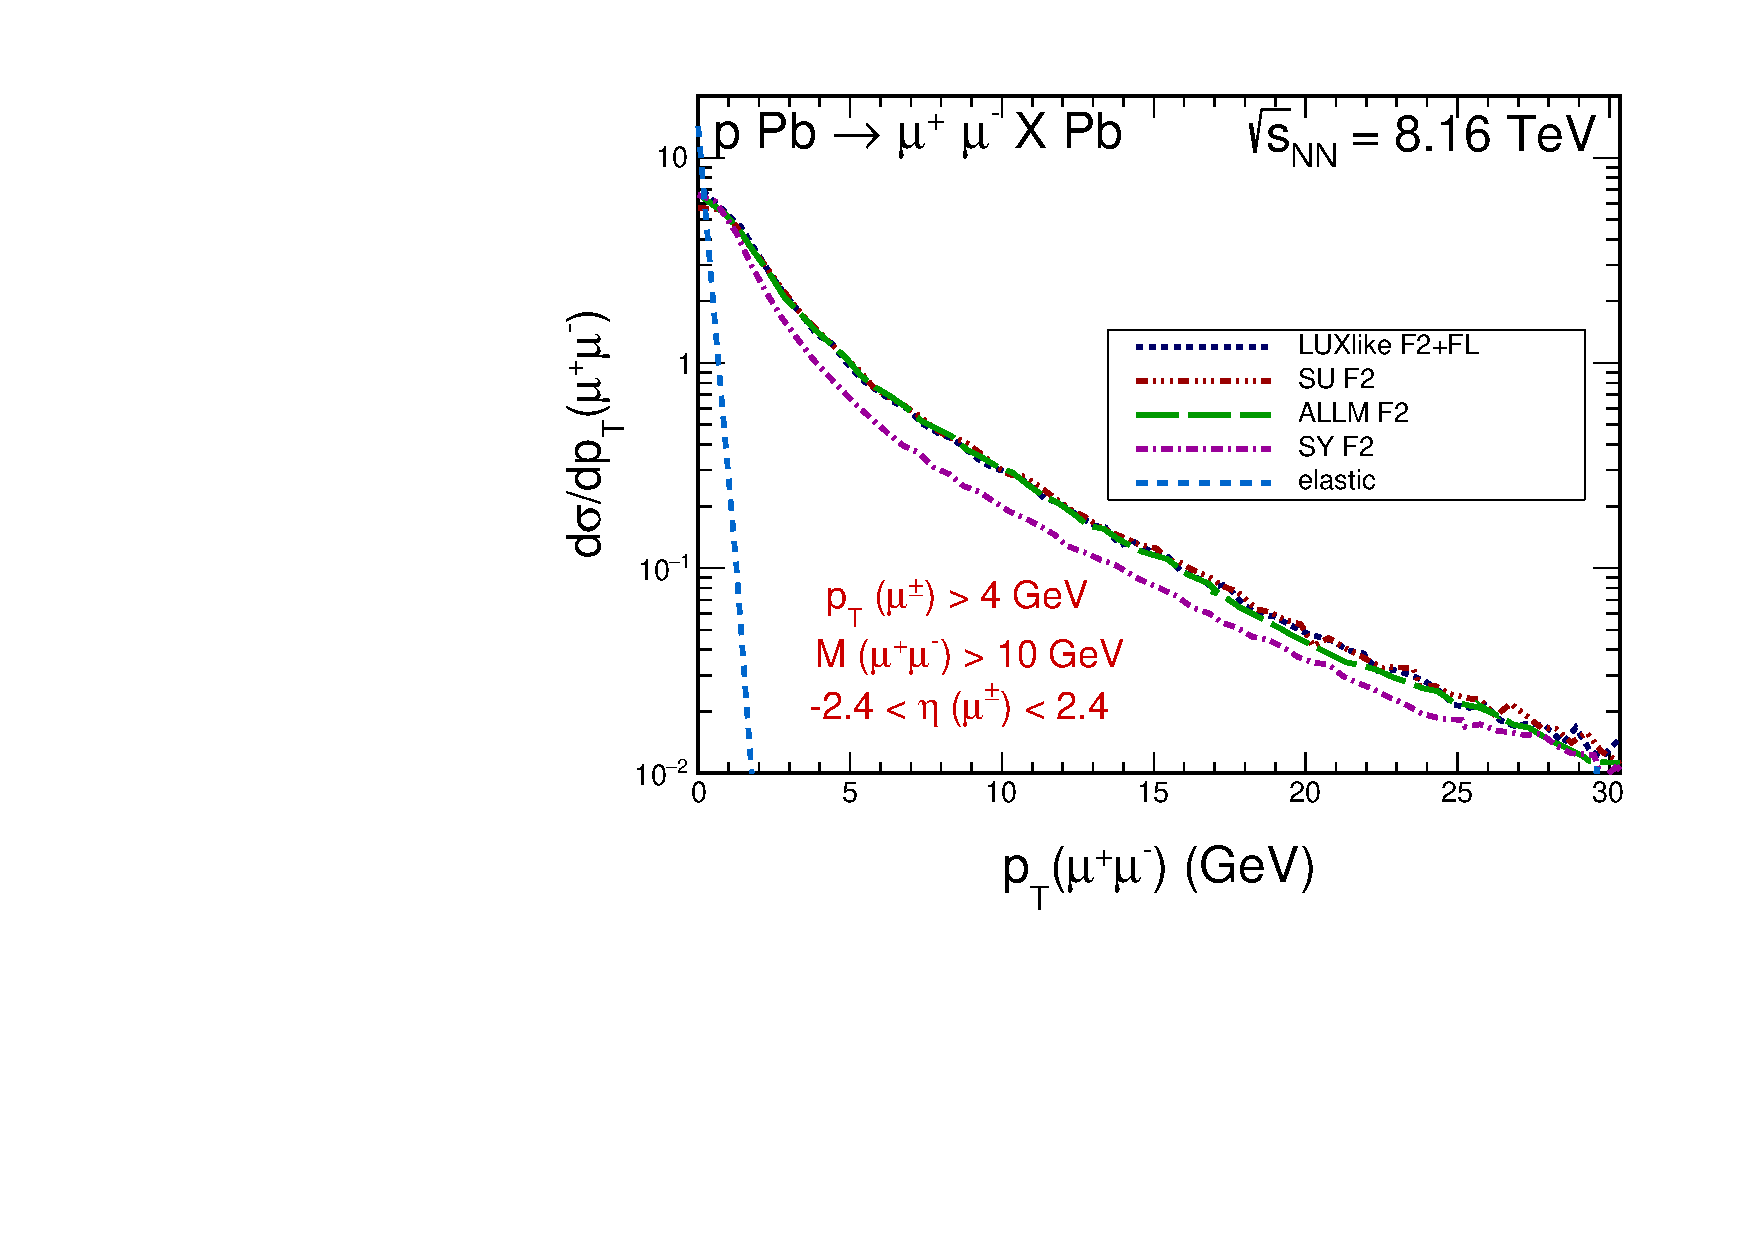
\includegraphics[width=0.49\textwidth]{figures/pt-sum-l.pdf}
 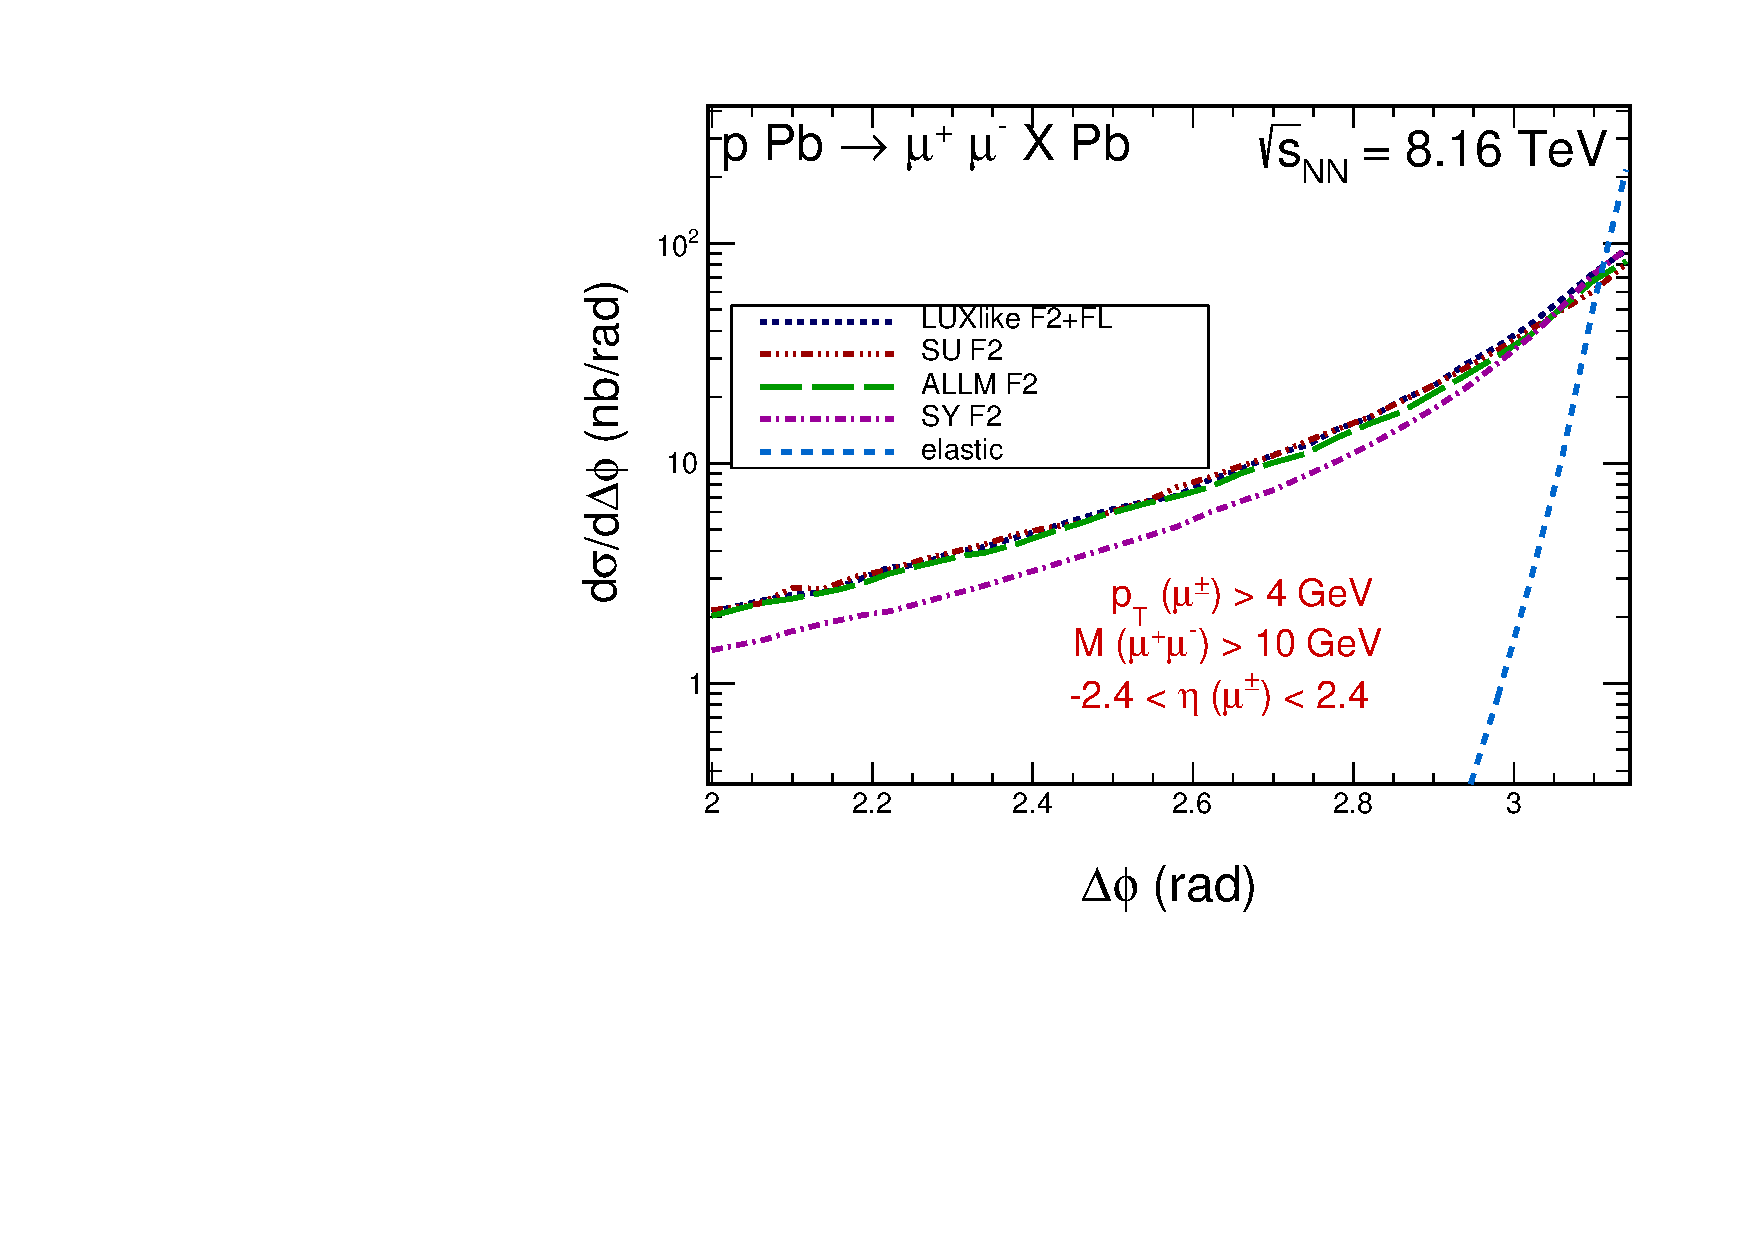
\includegraphics[width=0.49\textwidth]{figures/phi-l.pdf}
\caption{Differential cross sections in the fiducial region for $p+\textrm{Pb}\rightarrow \textrm{Pb} + \ell^+\ell^- + X$ production at $\sqrt{s_{N N}} = 8.16$~\TeV\ in $k_T$ factorization approach for several proton structure functions.
Two differential distributions are shown: transverse momentum of lepton pair (left) and azimuthal angle difference between the pair (right).
For comparison, the elastic contribution ($p+\textrm{Pb}\rightarrow p+ \textrm{Pb} + \ell^+\ell^-$) is also shown.
}
 \label{fig:kt_figures2}
\end{figure}
%------------------------------------------------------------------------------


%-----------------------------------------------------------------------------
\begin{figure}[!h]

 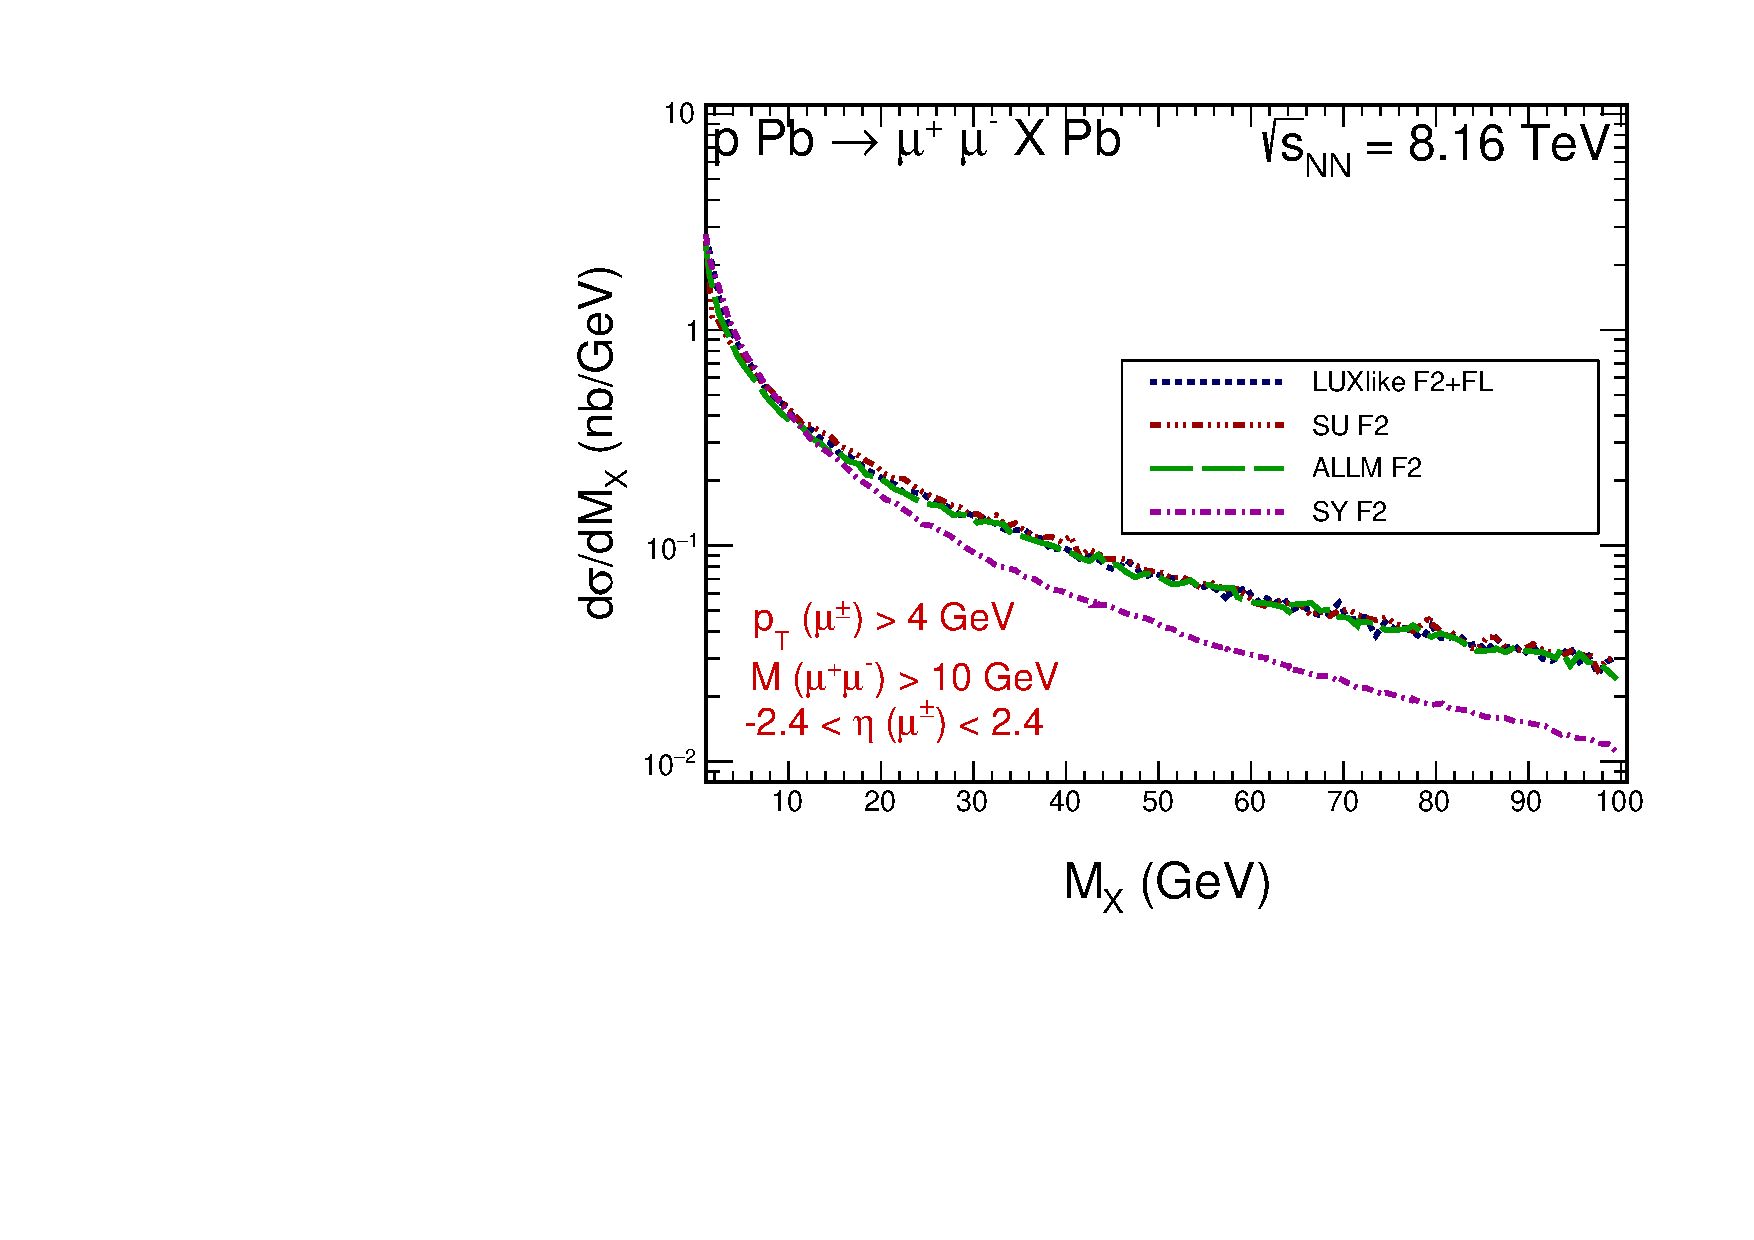
\includegraphics[width=0.49\textwidth]{figures/MX-l.pdf}
\caption{Differential cross section as a function of the mass of the proton remnants in the fiducial region for $p+\textrm{Pb}\rightarrow \textrm{Pb} + \ell^+\ell^- + X$ production at $\sqrt{s_{N N}} = 8.16$~\TeV\ in $k_T$ factorization approach for several proton structure functions.
}
 \label{fig:kt_figures3}
\end{figure}
%------------------------------------------------------------------------------






